\section{Blind simulation}
Blinds are automatically rolled up and down in order to simulate presence. They are rolled up and down using a semi random schema, in this case, the aperture of each blind is modified every hour.

To activate this characteristic go to BlindSimulation tab and click on the red button:
\begin{center}
	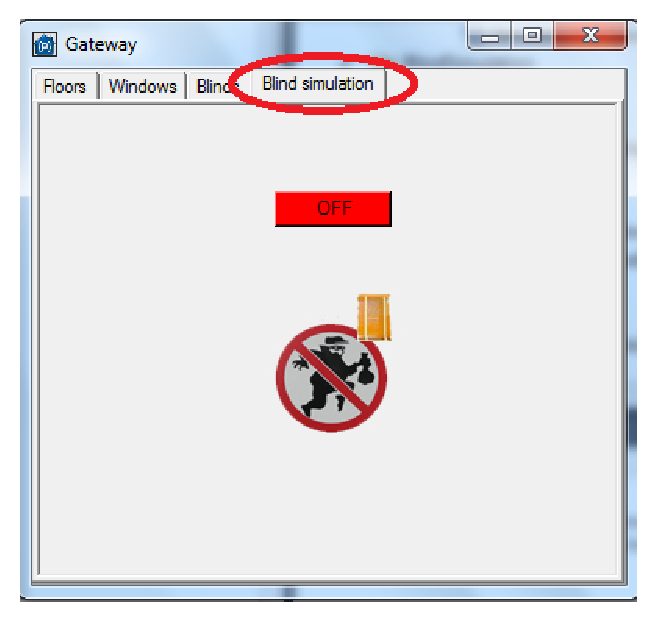
\includegraphics[width=.65\linewidth]{images/globalBlindSimulation.eps}
	\\
\vspace{1cm}
\end{center}

In the tag called BlindSimulation in the Simulator window, you can modified the current system time.
\begin{center}
	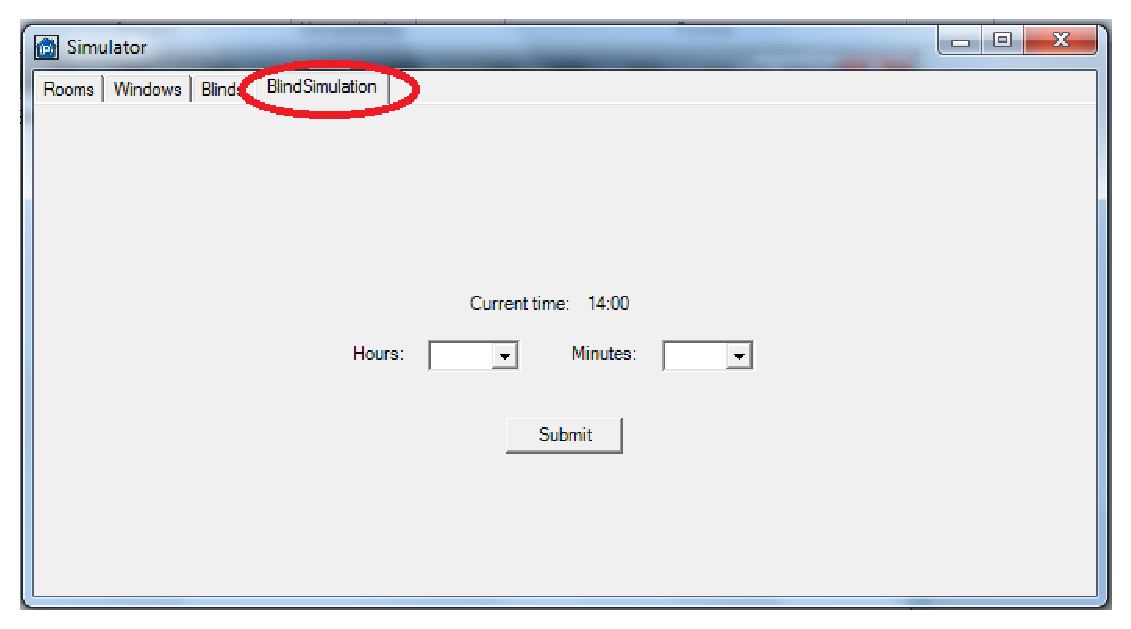
\includegraphics[width=.99\linewidth]{images/simulatorBlindSimulation.eps}
	\\
\vspace{1cm}
\end{center}

\end{document}